\documentclass[]{book}
\usepackage{subfiles}
\usepackage{exercise}
\usepackage{amsmath}
\usepackage{pgfplots}
\usepackage{import}
\usetikzlibrary{shapes,snakes}
%\usepackage{tikzpicture}
\begin{document}
\title{}
\author{Jigar Sura}
\date{}
\maketitle
\chapter{Root Finding}
\section{Bisection Method}
The bisection method is one of the iterative methods to find out real root of the continuous function of one variable. In this method, we first find the interval within which the root lies, i.e., the function crosses the x-axis. Let's learn this method with the help of a simple example. Let us say we wish to find out the square root of 2. We already know that $\sqrt{2} = 1.4142$. The function is $f(x) = x^{2}-2$. First step is to find out the interval where the root lies. The table below gives the value of the function for different values of $x$. 
\begin{center}
\begin{tabular}{|r|r|r|r|}
\hline
$x$ & 0 & 1 & 2\\
\hline
$f(x)$ & -2 & -1 & 2\\
\hline
\end{tabular}
\end{center}
\begin{figure}
\begin{center}
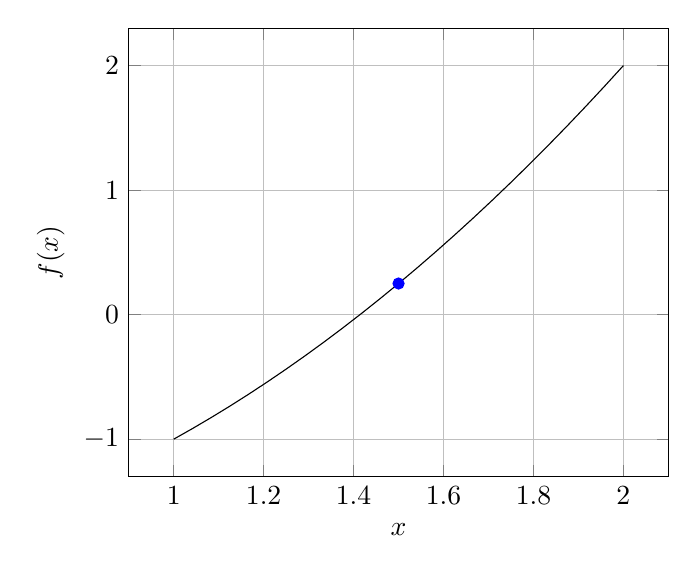
\begin{tikzpicture}
  \begin{axis}[ 
    xlabel=$x$,
    ylabel={$f(x)$},
    grid=major    
  ] 
    \addplot[domain=1:2] {x^2-2};
    \addplot[only marks,color=blue] plot coordinates {
        (1.5,0.25)};       
        
  \end{axis}
\end{tikzpicture}
\end{center}
\caption{Iteration 1}
\label{it1}
\end{figure}
As we can see, the function changes the sign between 1 and 2. Therefore, the root lies within $[1,2]$. So, we can safely assume that the root is at the midpoint of the interval, which means $\dfrac{1+2}{2} = 1.5$ can be the root of the function. The value of the function $f(1.5) = 0.25$. Table can be rewritten as follows.
\begin{center}
\begin{tabular}{|r|r|r|r|}
\hline
$x$ & 1 & 1.5 & 2\\
\hline
$f(x)$ & -1 & 0.25 & 2\\
\hline
\end{tabular}
\end{center}
The figure \ref{it1} shows the plot of the function.
Looking at the table, we can say that the root now lies within $[1,1.5]$ as the function changes the sign in this interval. Therefore, we can safely assume that the root is at the midpoint of the interval, which means $\dfrac{1+1.5}{2}=1.25$ can be the root of the function. The value of the function $f(1.25) = -0.4375$. Now, the table can be rewritten as follows.
\begin{center}
\begin{tabular}{|r|r|r|r|}
\hline
$x$ & 1 & 1.25 & 1.5\\
\hline
$f(x)$ & -1 & -0.4375 & 0.25\\
\hline
\end{tabular}
\end{center}
\begin{figure}
\begin{center}
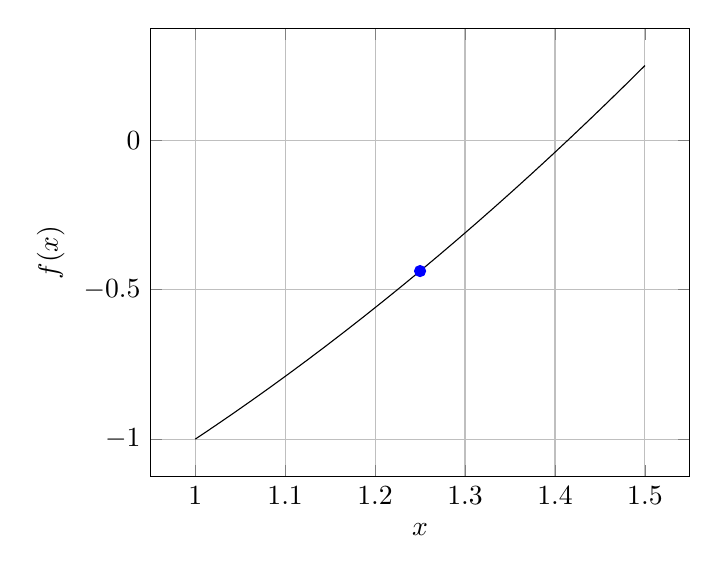
\begin{tikzpicture}
  \begin{axis}[ 
    xlabel=$x$,
    ylabel={$f(x)$},
    grid=major    
  ] 
    \addplot[domain=1:1.5] {x^2-2};
    \addplot[only marks,color=blue] plot coordinates {
        (1.25,1.25^2-2)};       
        
  \end{axis}
\end{tikzpicture}
\end{center}
\caption{Iteration 2}
\label{it2}
\end{figure}
The figure \ref{it2} shows the plot of the function. Following the above procedure again, we can say that the root now lies within $[1.25,1.5]$. The midpoint of this interval is 1.375. The value of the function $f(1.375) = -0.10938$. These steps can be summarized as follows for the implementation of the bisection method.
\begin{enumerate}
\item Determine the interval $[a,b]$ within which the root lies. The sign of the function are opposite to each other for these points, i.e. $f(a)\times f(b)<0$. 
\item Find the midpoint (say, $c$) of the interval and calculate the value of the function.
\item Based on the sign of the value of the function at midpoint, change $a$ or $b$ with $c$ such that $f(a)\times f(c)<0$ or $f(b)\times f(c)<0$.
\item If $f(a)\times f(c)<0$, replace $b$ with $c$ and repeat from the first step. Or if $f(b)\times f(c)<0$, replace $a$ with $c$ and repeat from the first step.
\end{enumerate}
\begin{ExerciseList}
\Exercise \textbf{Implement bisection method to solve $x^3-4x-9=0$.}
\Answer Let's find out where the function changes the sign, i.e., function crosses the x-axis.
\begin{center}
{\begin{tabular}{|r|r|r|r|r|}
\hline
$x$ & 0 & 1 & 2 & 3\\
\hline
$f(x)$ & -9 & -12 & -9 & 6\\
\hline
\end{tabular}}
\end{center}
As we can see, the function changes the sign between 2 and 3. Therefore, the root lies between $a=2$ and $b=3$. As per the method, the approximate root is 
$$ c = \frac{a+b}{2}=\frac{2+3}{2	}=2.5\ \&\ f(c) = -3.375$$
Since the signs of $f(c)$ and $f(a)$ are same, we will replace $a$ with $c$. So, now the root lies between $a = 2.5$ and $b = 3$. The approximate root is 
$$ c =  \frac{a+b}{2}=\frac{2.5+3}{2}=2.75\ \&\ f(c) = 0.79688$$
Since the signs of $f(c)$ and $f(b)$ are same, we will replace $b$ with $c$. So, now the root lies between $a = 2.5$ and $b = 2.75$. The approximate root is 
$$ c =  \frac{a+b}{2}=\frac{2.5+2.75}{2}=2.625\ \&\ f(c) = -1.41211$$
Writing in a tabular form
\begin{center}
\begin{scriptsize}
\begin{tabular}{|c|r|r|r|r|r|r|c|c|}
\hline
No. & $a$ & $f(a)$ & $b$ & $f(b)$ & $c=\frac{a+b}{2}$ & $f(c)$ & Replace & Error (\%)\\
\hline
1 & 2 & -9 & 3 & 6 & 2.5 & -3.375 & a & -\\
\hline
2 & 2.5 & -3.375 & 3 & 6 & 2.75 & 0.79688 & b & 9.09\\
\hline
3 & 2.5 & -3.375 & 2.75 & 0.79688 & 2.625 & -1.41211 & a & 4.76\\
\hline
4 & 2.625 & -1.41211 & 2.75 & 0.79688 & 2.6875 & -0.33911 & a & 2.33\\
\hline
5 & 2.6875 & -0.33911 & 2.75 & 0.79688 & 2.71875 & 0.22092 & b & 1.15\\
\hline
6 & 2.6875 & -0.33911 & 2.71875 & 0.22092 & 2.70313 & -0.060988 & a & 0.58\\
\hline
6 & 2.70313 & -0.060988 & 2.71875 & 0.22092 & 2.71094 & 0.079469 & b & 0.29\\
\hline
7 & 2.70313 & -0.060988 & 2.71094 & 0.079469 & 2.70704 & 9.2066E-3 & b & 0.14\\
\hline
8 & 2.70313 & -0.060988 & 2.70704 & 9.2066E-3 & 2.70509 & -0.025832 & a & 0.07\\
\hline
9 & 2.70509 & -0.025832 & 2.70704 & 9.2066E-3 & 2.70607 & -8.2304E-3 & a & 0.04\\
\hline
10 & 2.70607 & -8.2304E-3 & 2.70704 & 9.2066E-3 & 2.70656 & 5.7605E-4 & b & 0.02\\
\hline
\end{tabular}
\end{scriptsize}
\end{center}
Since the value of $c$ is repeated for 3 decimal points in the last two iterations, we can stop here. The root of the equation, therefore, is 2.70656.
\end{ExerciseList}
\subfile{bisection}
\subfile{FalsePosition}
\subfile{NewtonRaphson}
\chapter{Fitting of a straight Line}
\textbf{Fit $y = ae^{bx}$ for the data,}
\begin{center}
\begin{tabular}{|c|r|r|r|r|r|r|}
\hline
x & 2.30 & 3.10 & 4.00 & 4.92 & 5.91 & 7.20\\
\hline
y & 33.0 & 39.1 & 50.3 & 67.2 & 85.6 & 125.0\\
\hline
\end{tabular}
\end{center}
We have,
$$ y = ae^{bx}$$
Taking natural log both the sides,
$$ \underbrace{\ln y}_{Y} = \underbrace{\ln a}_{A} +bx$$
\begin{center}
\begin{tabular}{|r|r|r|r|r|r|}
\hline
No. & x & y & $Y = \ln y$ & $x^{2}$ & xY\\
\hline
1 & 2.3 & 33 &	3.4965 & 	5.29 & 8.042\\
\hline
2 & 3.1 & 	39.1 & 	3.6661 & 	9.61	 & 11.365\\
\hline
3 & 4 &	50.3 & 	3.9180 & 	16 & 	15.672\\
\hline
4 & 4.92 & 	67.2 & 	4.2077 & 	24.2064 & 	20.7018\\
\hline
5 & 5.91 & 	85.6 & 	4.4497 & 	34.9281 &	26.2976\\
\hline
6 & 7.2 & 	125 & 	4.8283 & 51.84 & 	34.7639\\
\hline
$\Sigma$ & 27.43 & 	400.2 & 	24.5663 & 	141.8745 & 	116.8422\\
\hline
\end{tabular}
\end{center}
The equations are
\begin{eqnarray}
\nonumber nA +b\Sigma x =& \Sigma Y\\
\nonumber A\Sigma x + b\Sigma x^{2} =& \Sigma xY
\end{eqnarray}
Inserting the values, we have
\begin{eqnarray}
\nonumber 6A + 27.43b =& 24.5663\\
\nonumber 27.43A + 141.8745b =& 116.8422
\end{eqnarray}
Solving above equations, we get $A =  2.8363$ \& $b = 0.2752$. Since $ A = \ln a$, we have $ a = e^{A} = 17.0533$. So, the equation of the curve is $$y=17.0533e^{0.2752x}$$
\subfile{linearcurve}
\chapter{Lagrange's formula}
\subfile{Lagrange}
\\ \textbf{Using Lagrange's formula, find the polynomial and evaluate $f(9)$.}
\begin{center}
\begin{tabular}{|c|r|r|r|r|r|}
\hline
$x$ & 5 & 7 & 11 & 13 & 17\\
\hline
$y$ & 150 & 392 & 1452 & 2366 & 5202\\
\hline
\end{tabular}
\end{center}
\begin{equation*}
\begin{aligned}
f(x) ={} &\frac{\left(x-x_{2}\right)\left(x-x_{3}\right)\left(x-x_{4}\right)\left(x-x_{5}\right)}{\left(x_{1}-x_{2}\right)\left(x_{1}-x_{3}\right)\left(x_{1}-x_{4}\right)\left(x_{1}-x_{5}\right)}y_{1}+\\
&\frac{\left(x-x_{1}\right)\left(x-x_{3}\right)\left(x-x_{4}\right)\left(x-x_{5}\right)}{\left(x_{2}-x_{1}\right)\left(x_{2}-x_{3}\right)\left(x_{2}-x_{4}\right)\left(x_{2}-x_{5}\right)}y_{2}+\\
&\frac{\left(x-x_{1}\right)\left(x-x_{2}\right)\left(x-x_{4}\right)\left(x-x_{5}\right)}{\left(x_{3}-x_{1}\right)\left(x_{3}-x_{2}\right)\left(x_{3}-x_{4}\right)\left(x_{3}-x_{5}\right)}y_{3}+\\
&\frac{\left(x-x_{1}\right)\left(x-x_{2}\right)\left(x-x_{3}\right)\left(x-x_{5}\right)}{\left(x_{4}-x_{1}\right)\left(x_{4}-x_{2}\right)\left(x_{4}-x_{3}\right)\left(x_{4}-x_{5}\right)}y_{4}+\\
&\frac{\left(x-x_{1}\right)\left(x-x_{2}\right)\left(x-x_{3}\right)\left(x-x_{4}\right)}{\left(x_{5}-x_{1}\right)\left(x_{5}-x_{2}\right)\left(x_{5}-x_{3}\right)\left(x_{5}-x_{4}\right)}y_{5}
\end{aligned}
\end{equation*}
\begin{equation*}
\begin{aligned}
f(x) ={} &\frac{\left(x-7\right)\left(x-11\right)\left(x-13\right)\left(x-17\right)}{\left(5-7\right)\left(5-11\right)\left(5-13\right)\left(5-17\right)}\times 150+\\
&\frac{\left(x-5\right)\left(x-11\right)\left(x-13\right)\left(x-17\right)}{\left(7-5\right)\left(7-11\right)\left(7-13\right)\left(7-17\right)}\times 392+\\
&\frac{\left(x-5\right)\left(x-7\right)\left(x-13\right)\left(x-17\right)}{\left(11-5\right)\left(11-7\right)\left(11-13\right)\left(11-17\right)}\times 1452+\\
&\frac{\left(x-5\right)\left(x-7\right)\left(x-11\right)\left(x-17\right)}{\left(13-5\right)\left(13-7\right)\left(13-11\right)\left(13-17\right)}\times 2366+\\
&\frac{\left(x-5\right)\left(x-7\right)\left(x-11\right)\left(x-13\right)}{\left(17-5\right)\left(17-7\right)\left(17-11\right)\left(17-13\right)}\times 5202
\end{aligned}
\end{equation*}
\begin{equation*}
\begin{aligned}
f(x) ={} &\frac{25}{192}\left(x^{4}-48x^{3}+838x^{2}-6288x+17017\right)-\\
&\frac{49}{60}\left(x^{4}-46x^{3}+756x^{2}-5186x+12155\right)+\\
&\frac{121}{24}\left(x^{4}-42x^{3}+616x^{2}-3702x+7735\right)-\\
&\frac{1183}{192}\left(x^{4}-40x^{3}+558x^{2}-3224x+6545\right)+\\
&\frac{289}{160}\left(x^{4}-36x^{3}+466x^{2}-2556x+5005\right)
\end{aligned}
\end{equation*}
\begin{equation*}
\Rightarrow \boxed{f(x) ={} x^{3}+x^{2}}
\end{equation*}
Now we will find $f(9)$.
$$f(9) = 9^{3}+9^{2} = 810$$
The figure \ref{lap2} shows the plot of the polynomial with given data.
\begin{figure}
\begin{center}
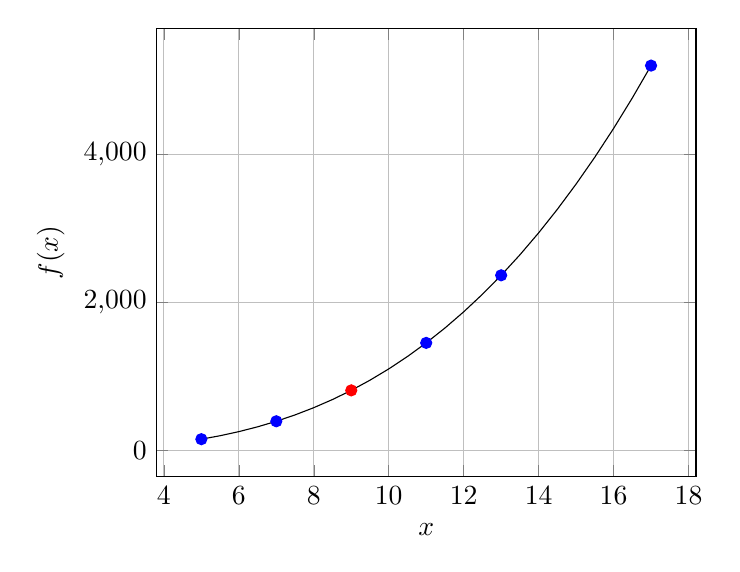
\begin{tikzpicture}
  \begin{axis}[ 
    xlabel=$x$,
    ylabel={$f(x)$},
    grid=major    
  ] 
    \addplot[domain=5:17] {x^3 + x^2};        
   \addplot[only marks,color=blue] plot coordinates {
        (5,150)
        (7,392)
        (11,1452)
        (13,2366)
        (17,5202)};  
        \addplot[only marks,color=red] plot coordinates {
        (9,810)};      
  \end{axis}
\end{tikzpicture}
\end{center}
\caption{Laplace interpolation}
\label{lap2}
\end{figure}

\chapter{Spline}
\textbf{Obtain cubic spline for every subinterval from the following data:}
\begin{center}
\begin{tabular}{|c|r|r|r|r|}
\hline
$x$ & 0 & 1 & 2 & 3\\
\hline
$y$ & 2 & -6 & -8 & 2\\
\hline
\end{tabular}
\end{center} 
This will require three cubics:
\begin{eqnarray}
S_{0}(x)=a_{0}+b_{0}(x-0)+c_{0}{(x-0)}^{2}+d_{0}{(x-0)}^{3}\\
S_{1}(x)=a_{1}+b_{1}(x-1)+c_{1}{(x-1)}^{2}+d_{1}{(x-1)}^{3}\\
S_{2}(x)=a_{2}+b_{2}(x-2)+c_{2}{(x-2)}^{2}+d_{2}{(x-2)}^{3}
\end{eqnarray}
Since there are 12 coefficients, we must derive 12 equations to solve. The splines must agree with the function at the nodes.
\begin{eqnarray}
2 = S_{0}(0) = a_{0}\\
-6 = S_{0}(1) = a_{0}+b_{0}+c_{0}+d_{0}\\
-6 = S_{1}(1) = a_{1}\\
-8 = S_{1}(2) = a_{1}+b_{1}+c_{1}+d_{1}\\
-8 = S_{2}(2) = a_{2}\\
2 = S_{2}(2) = a_{2}+b_{2}+c_{2}+d_{2}
\end{eqnarray}
The first and second derivatives of the cubics must agree at their shared nodes.
\begin{eqnarray}
S'_{0}(1) = b_{0}+2c_{0}+3d_{0} = b_{1} = S'_{1}(1)\\
S'_{1}(2) = b_{1}+2c_{1}+3d_{1} = b_{2} = S'_{2}(2)\\
S''_{0}(1) = 2c_{0}+6d_{0} = 2c_{1} = S''_{1}(1)\\
S''_{1}(2) = 2c_{1}+6d_{1} = 2c_{2} = S''_{2}(2)
\end{eqnarray}
The final two equations come from the natural boundary conditions.
\begin{eqnarray}
S''_{0}(0) = 0 = 2c_{0}\\
S''_{2}(3) = 0 = 2c_{2}+6d_{2}
\end{eqnarray}
All 12 linear equations together form the system:
\begin{eqnarray}
2 = & a_{0}\\
-6 = & a_{0}+b_{0}+c_{0}+d_{0}\\
-6 = & a_{1}\\
-8 = & a_{1}+b_{1}+c_{1}+d_{1}\\
-8 = & a_{2}\\
2 = & a_{2}+b_{2}+c_{2}+d_{2}\\
0 = & b_{0}+2c_{0}+3d_{0} - b_{1}\\
0 = & b_{1}+2c_{1}+3d_{1} - b_{2}\\
0 = & 2c_{0}+6d_{0} - 2c_{1}\\
0 = & 2c_{1}+6d_{1} - 2c_{2}\\
0 = & 2c_{0}\\
0 = & 2c_{2}+6d_{2}
\end{eqnarray}
The solution is
\begin{center}
\begin{tabular}{c|rrrr}
$i$ & $a_{i}$ & $b_{i}$ & $c_{i}$ & $d_{i}$\\
\hline
0 & 2 & -8.8 & 0 & 0.8\\
1 & -6 & -6.4 & 2.4 & 2\\
2 & -8 & 4.4 & 8.4 & -2.8
\end{tabular}
\end{center}
The natural cubic spline can be expressed as:
\begin{equation}
S(x) = \begin{cases} 2-8.8x+0.8x^{3} & \mbox{if } 0\leq x\leq 1\\
-6-6.4(x-1)+2.4{(x-1)}^{2}+2{(x-1)}^{3} & \mbox{if } 1\leq x\leq 2\\
-8+4.4(x-2)+8.4{(x-2)}^{2}-2.8{(x-2)}^{3} & \mbox{if } 2\leq x\leq 3\end{cases}
\end{equation}
The figure shows the plot of the spline with given data.
\begin{center}
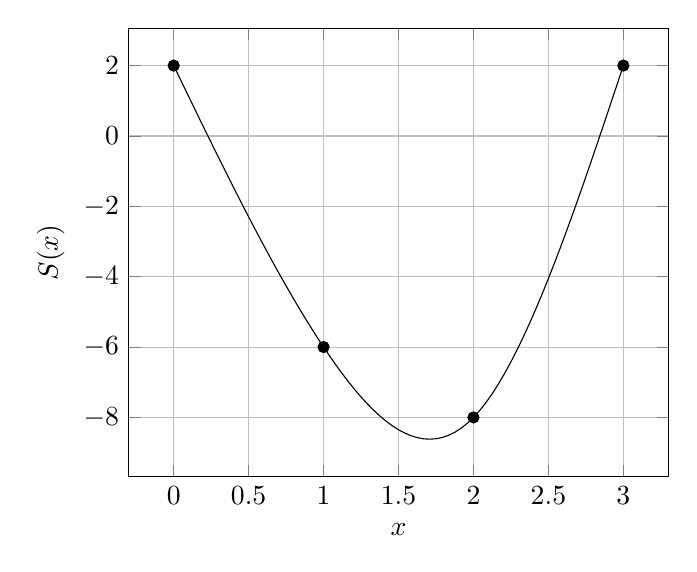
\begin{tikzpicture}
  \begin{axis}[ 
    xlabel=$x$,
    ylabel={$S(x)$},
    grid=major    
  ] 
    \addplot[domain=0:1] {2 - 8.8*x + 0.8*x^3};
    
        \addplot[domain=1:2] {-6-6.4*(x-1)+2.4*(x-1)^2+2*(x-1)^3};
        \addplot[domain=2:3] {-8+4.4*(x-2)+8.4*(x-2)^2-2.8*(x-2)^3};        
   \addplot[only marks] plot coordinates {
        (0,2)
        (1,-6)
        (2,-8)
        (3,2)};
        
  \end{axis}
\end{tikzpicture}
\end{center}
\chapter{Interpolation}
\textbf{Using  Newton's  forward  interpolation  formula,  find  the  value  of $f(1.6)$.}
\begin{center}
\begin{tabular}{|c|r|r|r|r|}
\hline
$x$ & 1 & 1.4 & 1.8 & 2.2\\
\hline
$f(x)$ & 3.49 & 4.82 & 5.96 & 6.5\\
\hline
\end{tabular}
\end{center}
\begin{center}
\begin{tabular}{r|rrrr}
$x$ & $f(x)$ & $\Delta y$ & ${\Delta}^{2} y$ & ${\Delta}^{3} y$\\
\hline
1 & 3.49 & & & \\
& & 1.33 & &\\
1.4 & 4.82 & & -0.19 &\\
& & 1.14 & & -0.41\\
1.8 & 5.96 & & -0.6 &\\
& & 0.54 & &\\
2.2 & 6.5 & & &\\
\end{tabular}
\end{center}
We have $x_{0} = 1$ and $h = x_{1}-x_{0} = 1.4 - 1 = 0.4$.\\
For $x = 1.6$, $$r=\dfrac{x-x_{0}}{h}=\dfrac{1.6-1}{0.4} = 1.5$$
$$f(x) = y_{0} + r\Delta y_{0}+\frac{r(r-1)}{2!}{\Delta}^{2}y_{0}+\frac{r(r-1)(r-2)}{3!}{\Delta}^{3}y_{0}$$
$$f(1.6) = 3.49+(1.5)(1.33)+\frac{(1.5)(0.5)}{2}(-0.19)+\frac{(1.5)(0.5)(-0.5)}{6}(-0.41)$$
$$\Rightarrow \boxed{f(1.6) = 5.439375}$$
\section{Stirling's formulae}
\textbf{Use Stirling's formulae for finding $y(12.2)$ from the data:}
\begin{center}
\begin{tabular}{|c|r|r|r|r|r|}
\hline
$x$ & 10 & 11 & 12 & 13 & 14\\
\hline
$y$ & 23967 & 28060 & 31788 & 35209 & 38368\\
\hline
\end{tabular}
\end{center}
\begin{center}
\begin{tabular}{r|rrrrr}
$x$ & $y$ & $\Delta y$ & ${\Delta}^{2} y$ & ${\Delta}^{3} y$ & ${\Delta}^{4} y$\\
\hline
10 & 23967 & & & & \\
& & 4093 & & &\\
11 & 28060 & & -365 & &\\
& & 3728 & & 58 &\\
12 & 31788 & & -307 & & -13\\
& & 3421 & & 45 &\\
13 & 35209 & & -262 & &\\
& & 3159 & & &\\
14 & 38368 & & & &
\end{tabular}
\end{center}
We have $x_{0} = 12$ and $h = x_{1}-x_{0} = 13 - 12 = 1$.\\
For $x = 12.2$, $$r=\dfrac{x-x_{0}}{h}=\dfrac{12.2-12}{1} = 0.2$$
\begin{equation*}
\begin{aligned}
f(x) = y_{0} +r\frac{\Delta y_{-1}+\Delta y_{0}}{2}+\frac{r^{2}}{2!}{\Delta}^{2}y_{-1}+ & \frac{r\left(r^{2}-1\right)}{3!}\frac{{\Delta}^{3}y_{-2}+{\Delta}^{3}y_{-1}}{2}+ \\ & \frac{r^{2}\left(r^{2}-1\right)}{4!}{\Delta}^{4}y_{-2}
\end{aligned}
\end{equation*}
\begin{equation*}
\begin{aligned}
f(12.2) = & 31788 +0.2\times\frac{3728+3421}{2}+\frac{0.2^{2}}{2!}(-307)+\\
& \frac{0.2(0.2^{2}-1)}{3!}\frac{58+45}{2}+\frac{0.2^{2}(0.2^{2}-1)}{4!}(-13)
\end{aligned}
\end{equation*}
$$ \Rightarrow f(12.2) = 31788+714.9 -6.14 -1.648 + 0.0208$$
$$\Rightarrow \boxed{f(12.2) = 32495.1328}$$
\chapter{Gauss Elimination Method}
Use Gauss elimination method to solve
\begin{eqnarray}
\nonumber x+4y-z=-5\\
\nonumber x+y-6z=-12\\
\nonumber 3x-y-z=4
\end{eqnarray} 
Writing in terms of $AX = B$, we have
$$A = \begin{bmatrix}
1 & 4 & -1\\
1 & 1 & -6\\
3 & -1 & -1
\end{bmatrix},\ X = \begin{bmatrix}
x\\ y\\ z
\end{bmatrix}\ \text{and}\ B = \begin{bmatrix}
-5\\ -12\\ 4
\end{bmatrix}$$
The augmented materix is
$$\begin{bmatrix}
1 & 4 & -1 & : & -5\\
1 & 1 & -6 & : & -12\\
3 & -1 & -1 & : & 4
\end{bmatrix}$$
Now, $R_{2}-R_{1}$ and $R_{3}-3R_{1}$, we get
$$\begin{bmatrix}
1 & 4 & -1 & : & -5\\
0 & -3 & -5 & : & -7\\
0 & -13 & 2 & : & 19
\end{bmatrix}$$
Now, $R_{3} - \frac{13}{3}R_{2}$, we get
$$\begin{bmatrix}
1 & 4 & -1 & : & -5\\
0 & -3 & -5 & : & -7\\
0 & 0 & 23.667 & : & 49.333
\end{bmatrix}$$
Therefore,
$$23.667z = 49.333 \Rightarrow z = 2.084$$
$$-3y-5z=-7 \Rightarrow y = -1.14$$
$$x+4y-z=-5 \Rightarrow x = 1.644$$
So, $X = \begin{bmatrix}
x\\ y\\ z \end{bmatrix} = \begin{bmatrix}
1.644\\ -1.14\\ 2.084
\end{bmatrix}$.\\
To check whether the answer is correct or not, we insert the values in given equations.
$$x+4y-z= 1.644+4(-1.14)-2.084 = -5$$
$$x+y-6z= 1.644-1.14-6(2.084) = -12$$
$$3x-y-z= 3(1.644)+1.14-2.084 = 3.988 \approx 4$$
\subfile{GaussElimination}
\input{GaussJordan}
\chapter{Integration}
\input{TrapezoidalRule}
\input{Simpson38}
\input{FDM}
\input{taylor}
\input{Picard}
\input{RungeKutta}
\subfile{shooting}
The End
\end{document}
